%
\chapter{Čas v podatkih na morju}
\label{sec:v_cas} 

Zgodovinsko, je bil čas v navigaciji eden od glavnih elementov določanja položaja. Čas so uporabljali za določanje zemljepisne dolžine ($\lambda$ ali ang. \emph{Longitude}). Pred izumom ure ali  kronometra (grško \emph{kronos} pomeni čas) je bila navigacija na morju zelo otežena. Le s pomočjo izmere razdalje so lahko napovedovali zemljepisno dolžino. Vsak si lahko predstavlja kakšno napako so pri tem storili. Prevoženo razdaljo so računali iz povprečne hitrosti, ki pa je bila obremenjena s hudo napako.

\begin{figure}[!h]
	\centering 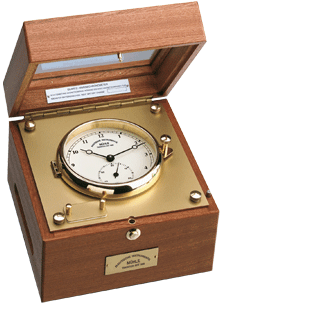
\includegraphics[width=8cm]{Vaje/CasPomorstvo/figs/kronometer_01.png}
	\caption{Navtični kronometer.}
\end{figure}

\section{Opis vaje}
\label{sec:v_cas_opis}
Namen vaje je seznanitev študenta z razumevanjem časa. Čas ima več oblik in natančnosti. Čas lahko merimo skozi ponavljajoče se astronomske dogodke (dan/noč, mesečeve mene, zenit sonca, $\ldots$), čakanje punce na želežniškem peronu, z atomsko uro in podobno. Skratka pojem časa je zelo relativen, zato je potrebno definirati kateri čas bomo uporabljali v tej nalogi.

\subsection{Dogovor o zapisu in uporabi časa:}
\begin{itemize}
	\item \textsc{Format zapisa}:\\[2mm]
	Čas bomo zapisovali v obliki\\[2mm] 
	\textbf{HH:MM:SS.ss},\\[2mm]
	kjer je \textbf{H}-ura, \textbf{M}-minuta, \textbf{S}-sekunda in \textbf{s}-delež sekunde v decimalni obliki. Natančnost časovne meritve bomo vedno zapisali na dve decimalki natančno. Kot primer zapišimo:\\[2mm] 
	%
	13:12:10.33 - 13h, 12min, 10.33sek; urni zapis je v 24h\\
	%
	\item \textsc{Časovna zona}:\\[2mm]
	Enako je potrebno definirati v kateri časovni zoni bomo čas zapisovali. Vedno je potrebno čas zapisati v UTC. Za podrobnosti, kaj UTC pomeni si poglejte na splet\\[2mm] \url{https://en.wikipedia.org/wiki/Coordinated_Universal_Time}\\
	
	\item \textsc{Časovna referenca}:\\[2mm]
	Za časovno referenco vzemite enega od časovnih strežnikov, kot na primer:\\[2mm]
	\url{http://www.ijs.si/time/ijs-time.html}\\[2mm]
	Tako boste imeli svoje elektronske naprave dobro sinhronizirane.\\
\end{itemize}

Kot smo videli imamo v dogovoru definirano uporabo časovne reference. Čas venomer prislonimo na določeno časovno referenčno točko. Danes večino meritev v pomorstvu sinhroniziramo prav s časom, ki ga dobimo iz GPS sprejemnika. Sateliti, ki jih uporabljamo za določanje položaja imajo izjemno natančen čas, ki ga lahko spremljamo na GPS sprejemniku.



\subsection{Izvedba vaje}
Izvedba vaje bo potekala v dveh delih. V prvem delu je potrebno narediti daljši poizkus, ki bo zajemal slikanje večjega števila ur in primerjavo časa med njimi. V drugem delu bo potrebno s pomočjo natančnega časa določiti geografsko dolžino.

\subsubsection{Spremljanje različnih ur}
V tem poizkusu, je potrebno zbrati najmanj 5 različnih analognih ur (tiste s kazalci). Postavite jih na skupen prostor, da jih boste lahko slikali skupaj. Poleg vedno pristavite še telefon ali tablico, ki bo imela čas sinhroniziran na enega od časovnih strežnikov, da boste točno vedeli kakšen je točen čas. Čas iz tablice ali telefona imate kot točno časovno referenco. 

Slikati je potrebno vsak dan in sicer v obdobju 14 dni. Na koncu zberite slike skupaj, obdelajte podatke in jih vnesite v tabelo. Tabela naj vsebuje točen čas in čas ostalih ur, razliko ur od točnega časa in napako meritve odčitka časa na analogni uri.

\begin{table}
	\centering
	\caption{Meritve časovnih zamikov za dan 21.09.2015}
	\label{tab:v_cas_meritev} 
	\begin{tabular}{l||c|r|r}
		\hline
		ura & čas & napaka & razlika  \\
	    \hline\hline\noalign{\smallskip}
		1.  & 13:45:22 & 1s   & 3s\\
		2.  & 13:46:30 & 30s  & 5s\\
		ref & 13:45:25 & 0.5s & - 
	\end{tabular}
\end{table}

\subsubsection{Določitev zemljepisne dolžine}
Zemljepisno dolžino je moč določiti s pomočjo meritve časa, ko je Sonce v zenitu. Za izvedbo te vaje je potrebno sestaviti primitivno napravo, s katero boste lahko natančno odčitali višino Sonca.\\[2mm]
%
\textbf{Pozor! Nikoli ne poglejte v Sonce s prostim očesom. Vedno morate oko zaščititi s primernim filtrom!}\\[2mm]
%
Recimo primitiven višinomer s pomočjo kota je lahko nekaj podobnega tistemu, kar je prikazano na sliki \ref{fig:v_cas_kotomer}. Natančnost odmerka višine je pogojena z dolžino letvice, ki dela senco Sonca. Daljša kot je širša je senca in s tem natančnejša je naša meritev. 
%
\begin{figure}[!htbp]
	\centering 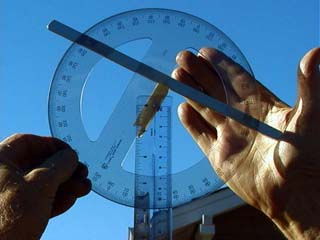
\includegraphics[width=8cm]{Vaje/CasPomorstvo/figs/kotomer.jpg}
	\caption{Primitiven kotomer.}
	\label{fig:v_cas_kotomer}
\end{figure}
%
Kako pa določimo zemljepisno dolžino - $\lambda$?\\[2mm]
%
Med premikanjem kotomera, merimo tudi točen čas. Ko ugotovimo, da se Sonce ne dviga več in se je pričelo spuščati, zabeležimo čas, ko je Sonce najvišje ali v \emph{zenitu}. Ne pozabimo, čas je v UTC.\\[2mm]
%
Čas merimo s srednjim Sončnim časom. Pravi Sončni čas je mera s katerim lahko indentificiramo našo geografsko širino $\lambda$. Razlika med pravim Sončnim časom in srednjim Sončnim časom je \emph{časovna enačba}. To je količina, ki se med letom spreminja in jo dobimo v navtičnem almanahu. Formula po kateri določimo $\lambda$ je:

\begin{equation}
\label{eq:v_cas_lambda} 
\lambda[\si{\degree}] := 15\si{\degree} \left( \text{LT}_{\text{kulminacije}} - 12h + \eta(\text{UTC}) \right).
\end{equation}

Paziti moramo, da je čas, ki ga vnesemo v enačbo (\ref{eq:v_cas_lambda}) vedno v urah. Torej moramo čas, ki je zapisan HH:MM:SS pretvoriti v HH.hhhh. Nato s pomočjo enačbe (\ref{eq:v_cas_lambda}) lahko določimo našo zemljepisno dolžino v stopinjah. Kratice pomenijo: LT - local time, $\eta(\text{UTC})$ časovna enačba podana v navtičnem almanahu, kjer je parameter UTC.

Časovno enačbo in oceno, kdaj je sonce v kulminaciji si lahko določite na strani \href{https://www.esrl.noaa.gov/gmd/grad/solcalc/azel.html}{Solar Position Calculator} ali še z grafičnim prikazom na strani \href{https://www.esrl.noaa.gov/gmd/grad/solcalc/}{NOAA Solar Calculator}. Na sliki \ref{fig:v_cas_calculator} je prikazan vnos podatkov in določitev časovnega popravka ($\eta$ - Equation of Time) z časom in višino sonca.
%
\begin{figure}[tbph!]
	\centering 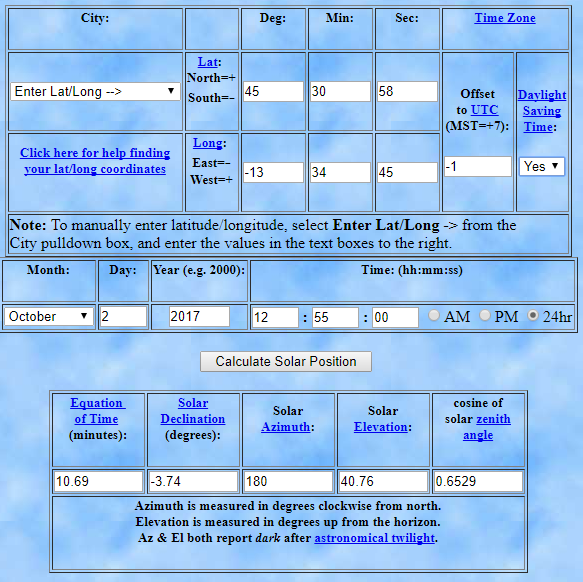
\includegraphics[width=8cm]{Vaje/CasPomorstvo/figs/calculator.png}
	\caption{Okno v katerim vnesete parametre za določitev časovnega popravka in ocena ure kulminacije Sonca.}
	\label{fig:v_cas_calculator}
\end{figure}

%
Odogovori na naslednja vprašanja:\\[2mm]
V enačbi (\ref{eq:v_cas_lambda}) se predznak $\lambda$ spremeni, ko je sonce v zenitu po 12h UTC. Kaj to pomeni? Kje smo, ko je sonce v zenitu točno ob 12h UTC? Pa še to, kaj je datumska meja?

\section{Zanimivosti uporabe časa}
Za tiste, ki ste bolj astronomsko navdahnjeni, pa priporočam uporabo časa in navtičnega almanaha za identificiranje zvezdnega neba. Lepa stran, ki vam kaže severno nebo je:\\[2mm]
%
\href{http://www.jodcast.net/sky}{nočno nebo nad nami}
%
